% !TEX root = ../main.tex

\section{Experiments}
\subsection{Datasets}
\label{sec:5.1}
We evaluate our method on two standard action anticipation benchmarks: the Breakfast dataset and 50 Salads.

The Breakfast~\cite{kuehne2014language} dataset comprises 1,712 videos of 52 different individuals cooking breakfast in 18 different kitchens.
Every video is categorized into one of the 10 activities related to breakfast preparation.
There exist 48 fine-grained action labels which are used to make up the activities.
On average, each video is about 2.3 minutes long and includes approximately 6 actions.
All videos were down-sampled to a resolution of 240$\times$320 pixels with a frame rate of 15 fps.
The dataset comprises 4 splits of training and test set, and we report the average performance over all the splits following the previous work~\cite{abu2018will,sener2020temporal,farha2020long}.

The 50 Salads~\cite{stein2013combining} dataset comprises 50 videos of 25 people preparing a salad. The dataset contains over 4 hours of RGB-D video data, annotated with 17 fine-grained action labels and 3 high-level activities. Since 50 Salads is usually longer than Breakfast, each video contains 20 actions on average. Every video in the dataset has a resolution of 480$\times$640 pixels with a frame rate of 30 fps. The dataset comprises 5 splits of training and test set, and we report the average results over all the splits.
% \vspace{-3mm}

\subsection{Implementation details}
\label{sec:5.2}
\noindent
\textbf{Architecture details.}
Our model consists of two encoder layers and one decoder layer for Breakfast and two encoder layers and two encoder layers for 50 Salads. 
We set the number of object queries $M$ to 8 for Breakfast and 20 for 50 Salads since 50 Salads includes more actions than Breakfast in a video.
The size of hidden dimension $D$ is set to 128 for Breakfast and 512 for 50 Salads.

\noindent
\textbf{Training \& testing.}
We use pre-extracted I3D features\cite{carreira2017quo} as input visual features for both Breakfast and 50 Salads provided by~\cite{farha2019ms}.
We sample the I3D features with a stride $\tau$ of 3 for Breakfast and 6 for 50 Salads.
In training, we set the observation rate $\alpha \in \{0.2, 0.3, 0.5\}$ and fix the prediction rate $\beta$ to 0.5. 
We use AdamW optimizer\cite{loshchilov2017decoupled} with a learning rate of 1e-3.
We train our model for 60 epochs with a batch size of 16, employing a cosine annealing warm-up scheduler\cite{loshchilov2016sgdr} with warm-up stages of 10 epochs.
In inference, we set the observation rate $\alpha \in \{0.2, 0.3\}$ and prediction rate $\beta \in \{0.1, 0.2, 0.3, 0.5\}$ and measure mean over classes~(MoC) accuracy following the long-term action anticipation framework protocol~\cite{abu2018will,ke2019time,sener2020temporal,farha2020long}.

\subsection{Comparison with the state of the art}
\label{sec:5.3}
In Table~\ref{tab:sota}, we compare our methods with the state-of-the-art methods on Breakfast and 50 Salads.
The table is divided into two compartments according to the dataset, and each compartment is divided into two sub-compartments according to the input types;
the first and the second sub-compartment utilize action labels extracted from the action segmentation model~\cite{richard2017weakly} and visual features, respectively.
For Breakfast, CNN~\cite{abu2018will} uses the Fisher vectors~\cite{abu2018will}, and the other models use I3D features~\cite{carreira2017quo} as input.
For 50 Salads, Sener~\etal~\cite{sener2020temporal} use the Fisher vectors and Farha~\etal~\cite{farha2020long} use I3D features.
As a result, our methods achieve the state-of-the-art performance in all experimental settings on Breakfast and 6 out of 8 settings on 50 Salads, respectively, using visual features only.

\subsection{Analysis}
\label{sec:5.4}
We conduct in-depth analyses to validate the efficacy of the proposed method. In the following experiments, we evaluate our method on the Breakfast dataset setting the observation ratio $\alpha$ as 0.3.
Unless otherwise specified, all experimental settings are the same as those in Sec.~\ref{sec:5.2}.
Further experimental details are indicated in Supp.~A.

\begin{table}[t!]
\begin{center}
\scalebox{0.76}{
\begin{tabular}{C{1.5cm}C{0.5cm}C{1cm}C{0.9cm}C{0.9cm}C{0.9cm}C{0.9cm}C{0.9cm}}
        % \cmidrule[1.0pt]{1-7}
        \toprule
        \multirow{2}*[-0.5ex]{method}&\multirow{2}*[-0.5ex]{AR}& \multirow{2}*[-0.5ex]{\shortstack{causal \\ mask}} & \multicolumn{4}{c}{$\beta~(\alpha=0.3)$} & \multirow{2}*[-0.5ex]{\shortstack{time\\(ms)}}\\
        % \cmidrule[0.8pt]{3-6}
        \cmidrule{4-7}
        &&& 0.1 & 0.2 & 0.3 & 0.5 & \\
        \midrule
        \ours-A &\checkmark&\checkmark& 27.10 & 25.41 & 23.28 & 20.51 & 14.68\\
        \ours-M &-&\checkmark& 31.82 & 28.55 & 26.57 &  24.17 & 5.70\\
        \ccolg \ours &\ccolg-&\ccolg-& \ccolg\textbf{32.27} &\ccolg\textbf{29.88} & \ccolg\textbf{27.49} &  \ccolg\textbf{25.87} & \ccolg \textbf{3.91}\\
        % \cmidrule[1.0pt]{1-7}
        \bottomrule
        \end{tabular}
        }
% \vspace{-2mm}
\caption{\textbf{Parallel decoding vs. autoregressive decoding.}  Parallel decoding significantly improves both accuracy and inference speed. \ours-A autoregressively anticipates future actions using predicted action labels with masked self-attention, and \ours-M anticipates future actions using action queries with masked self-attention. 
All the reported inference speeds are measured on a single RTX 3090 GPU, ignoring data loading time. We feed a single video on GPU and take an average on the test set, except the first ten samples as a warm-up stage for stable inference time~\cite{lin2019tsm}.}
\label{tab:parallel}
\end{center}
\vspace{-4mm}
\end{table}
% C{0.75cm}C{1cm}C{0.9cm}C{0.9cm}C{0.9cm}C{0.9cm}C{0.9cm}

\vspace{1mm}

\noindent
\textbf{Parallel decoding vs. autoregressive decoding.}
To validate the effectiveness of parallel decoding for long-term action anticipation, we compare our method with two \ours variants with different decoding strategies.
The first variant \ours-A autoregressively anticipates future actions similar to transformer~\cite{vaswani2017attention}. \ours-A takes the output action labels from the previous predictions as input and utilizes masked self-attention. Masked self-attention employs a causal mask to MHSA, which prevents attending to future actions.
The second variant \ours-M is equivalent to \ours except for masked self-attention applied to action queries. \ours-M takes the action queries as input and predicts future actions in parallel, but each query only attends to the past queries.

Table~\ref{tab:parallel} summarizes the results.
FUTR-M outperforms FUTR-A by 3.1-4.7\%p, with 2.6$\times$ faster inference time.
These results demonstrate the effectiveness of parallel decoding using action queries in terms of accuracy and efficiency.
As we remove the causal mask from \ours-M, we obtain an additional accuracy improvement of 0.4-1.7\%p.
Compared to \ours-A, \ours achieves higher accuracy by 4.2-5.4\%p, inferring 3.8$\times$ faster.
These results show the effectiveness of parallel decoding of leveraging bi-directional dependencies between action queries leading to a more accurate and faster inference.
\begin{table}[t!]
\begin{center}
\scalebox{0.9}{
\begin{tabular}{C{1.3cm}C{1.3cm}C{1cm}C{1cm}C{1cm}C{1cm}}
        \toprule
        \multirow{2}*[-0.5ex]{encoder}& \multirow{2}*[-0.5ex]{decoder} & \multicolumn{4}{c}{$\beta~ (\alpha=0.3)$}\\
        \cmidrule{3-6}
        && 0.1 & 0.2 & 0.3 & 0.5 \\
        \cmidrule{1-6}
        LSA&LSA& 27.70 & 24.39 & 23.18 &  21.60\\
        GSA&LSA& 30.15 & 27.51 & 25.62 &  23.28\\
        LSA&GSA& 28.37 & 25.08 & 24.03 &  22.28\\
        \ccolg GSA&\ccolg GSA& \ccolg \textbf{32.27} &\ccolg \textbf{29.88} & \ccolg\textbf{27.49} &  \ccolg\textbf{25.87}\\
        \bottomrule
        \end{tabular}
        }
% \vspace{-2mm}
\caption{\textbf{Global self-attention vs. local self-attention.} Using GSA in both the encoder and the decoder improves the performance, indicating that learning long-term dependencies not only between the observed frames but also between the possible future actions is important for long-term action anticipation.}
\label{tab:locality}
\end{center}
\vspace{-2mm}
\end{table}
% C{1.3cm}C{1.3cm}C{1cm}C{1cm}C{1cm}C{1cm}

\vspace{1mm}
\noindent
\textbf{Global self-attention vs. local self-attention.}
We investigate the effect of learning long-term temporal dependencies between past and future actions by comparing global self-attention~(GSA) and local self-attention~(LSA)~\cite{ramachandran2019stand}.
We build a \ours variant that computes LSA in both the encoder and the decoder, and then replaces LSA with GSA one by one.
We set the window sizes of LSA in the encoder and the decoder as 201 and 3, respectively, where only local area within the window size is utilized for MHA.

The results in Table~\ref{tab:locality} validate the efficacy of using GSA in long-term action anticipation.
From the $1^{\textrm{st}}$ and $2^{\textrm{nd}}$ rows, we observe that replacing LSA with GSA in the encoder improves the accuracy by 1.7-3.1\%p. 
The result verifies that learning the global context between past frames is crucial.
As we replace LSA with GSA in the decoder from the $1^{\textrm{st}}$ and $3^{\textrm{rd}}$ rows, we find consistent accuracy improvement by 0.7-0.9\%p.
We find that learning global temporal relations between action queries is also essential for anticipating a sequence of future actions.
Finally, we replace all LSA to GSA in both the encoder and the decoder from the $1^{\textrm{st}}$ and $4^{\textrm{th}}$ rows, which brings significant improvements by 4.3-5.5\%p, achieving the best accuracy.
These results demonstrate the importance of learning long-term relations between the observed actions in the past and potential actions in the future.

% \vspace{3mm}
\begin{table}[t!]
\begin{center}
\scalebox{0.77}{
\begin{tabular}{C{1.4cm}C{1.65cm}C{1.6cm}C{0.8cm}C{0.8cm}C{0.8cm}C{0.8cm}}
        \toprule
        \multirow{2}*[-0.5ex]{method}&\multirow{2}*[-0.5ex]{GT Assign.}&\multirow{2}*[-0.5ex]{regression} &  \multicolumn{4}{c}{$\beta~(\alpha=0.3)$}\\
        \cmidrule{4-7}
        &&& 0.1 & 0.2 & 0.3 & 0.5 \\
        \midrule
        \ours-S & sequential  & start-end & 29.15 & 25.51 & 24.20 & 21.43\\
        \ours-H & Hungarian &start-end & 25.26 & 23.85 & 22.63 & 21.45\\
        \ccolg\ours & \ccolg sequential & \ccolg duration & \ccolg\textbf{32.27} &\ccolg\textbf{29.88} & \ccolg\textbf{27.49} &  \ccolg\textbf{25.87}\\
        \bottomrule
        \end{tabular}
        }
% \vspace{-2mm}
\caption{\textbf{Output structuring.}
\ours shows the superior performance over \ours-S and \ours-H. We find that sequential order of the ground truth assignment and duration regression is effective for long-term action anticipation.
% Setting the temporal orders of the action queries helps the model consider temporal relations between actions.
% Fixing the temporal position of the action queries with duration regression dramatically increase the performance. 
Start-end regression predicts normalized start and end timestamp for each query instead of the duration.
}
\label{tab:setpred}
\end{center}
\vspace{-6mm}
\end{table}

% \begin{table}[t!]
% \begin{center}
% \scalebox{0.73}{
% \begin{tabular}{C{1.8cm}C{1.7cm}C{1.6cm}C{0.8cm}C{0.8cm}C{0.8cm}C{0.8cm}}
%         \toprule
%         \multirow{2}*[-0.5ex]{Method}&\multirow{2}*[-0.5ex]{GT Assign.}&\multirow{2}*[-0.5ex]{Regression} &  \multicolumn{4}{c}{$\beta~(\alpha=0.3)$}\\
%         \cmidrule{4-7}
%         &&& 0.1 & 0.2 & 0.3 & 0.5 \\
%         \midrule
%         \multirow{2}*[-0.5ex]{Hungarian \ours} & Hungarian &start-end & 25.26 & 23.85 & 22.63 & 21.45\\
%         Start-end \ours & sequential  & start-end & 29.15 & 25.51 & 24.20 & 21.43\\
%         \ccolg\ours & \ccolg sequential & \ccolg duration & \ccolg\textbf{32.27} &\ccolg\textbf{29.88} & \ccolg\textbf{27.49} &  \ccolg\textbf{25.87}\\
%         \bottomrule
%         \end{tabular}
%         }
% \vspace{-2mm}
% \caption{\textbf{Output regression.}
% \dygong{\ours show superior performance over the Hungarian \ours and Start-end \ours.} Setting the temporal orders of the action queries helps model consider temporal relations between actions.
% % Fixing the temporal position of the action queries with duration regression dramatically increase the performance. 
% Start-end regression predicts normalized start and end timestamp for each query instead of the duration.
% }
% \label{tab:setpred}
% \end{center}
% \vspace{-6mm}
% \end{table}
% C{1.95cm}C{1.9cm}C{0.8cm}C{0.8cm}C{0.8cm}C{0.8cm}

% \begin{table}[t!]
% \begin{center}
% \scalebox{0.74}{
% \begin{tabular}{C{1.6cm}C{1.65cm}C{1.6cm}C{0.8cm}C{0.8cm}C{0.8cm}C{0.8cm}}
%         \toprule
%         \multirow{2}*[-0.5ex]{Method}&\multirow{2}*[-0.5ex]{GT Assign.}&\multirow{2}*[-0.5ex]{regression} &  \multicolumn{4}{c}{$\beta~(\alpha=0.3)$}\\
%         \cmidrule{4-7}
%         &&& 0.1 & 0.2 & 0.3 & 0.5 \\
%         \midrule
%         \multirow{2}*[1ex]{Hungarian} & \multirow{2}*{Hungarian} & \multirow{2}*{start-end} & \multirow{2}*{25.26} & \multirow{2}*{23.85} & \multirow{2}*{22.63} & \multirow{2}*{21.45}\\
%         \ours & & & & & & \\
%         \multirow{2}*[1ex]{Start-end} & \multirow{2}*{sequential}  & \multirow{2}*{start-end} & \multirow{2}*{29.15} & \multirow{2}*{25.51} & \multirow{2}*{24.20} & \multirow{2}*{21.43}\\
%         \ours & & & & & & \\
%         \ccolg\ours & \ccolg sequential & \ccolg duration & \ccolg\textbf{32.27} &\ccolg\textbf{29.88} & \ccolg\textbf{27.49} &  \ccolg\textbf{25.87}\\
%         \bottomrule
%         \end{tabular}
%         }
% \vspace{-2mm}
% \caption{\textbf{Output regression.}
% \dygong{\ours shows the superior performance over the Hungarian \ours and Start-end \ours. We find that sequential order of the ground truth assignment and duration regression is effective for long-term action anticipation.}
% % Setting the temporal orders of the action queries helps the model consider temporal relations between actions.
% % Fixing the temporal position of the action queries with duration regression dramatically increase the performance. 
% Start-end regression predicts normalized start and end timestamp for each query instead of the duration.
% }
% \label{tab:setpred}
% \end{center}
% \vspace{-6mm}
% \end{table}
%%%%%%%%%%%%%%%%%%%%%%%%%%%%%%%%%%%%%%%%%%%%%%%%%%%%%%%%%%
\noindent
\textbf{Output structuring.}
To obtain the final output, we consider the action queries as an ordered {\it sequence} and train FUTR to predict an action label and its duration from each in the sequence of action queries; in training, the ground truths of label and duration are directly assigned to the outputs of the queries in the sequential order.
To validate the effectiveness of this output structuring strategy, we compare it with two FUTR variants with different output structuring methods.
\ours-S is a variant of our method that is trained to predict a temporal window of starting and ending points, instead of a duration, from each in the query sequence. 
In inference, the predicted start-end windows are merged with priority according to classification logits; the most confident action labels are assigned to overlapping regions of windows. 
\ours-H is a DETR-like variant~\cite{carion2020end} that considers the action queries as an unordered {\it set}, not a sequence, and predicts a start-end window from each in the query set. In training, the ground truths are assigned to the outputs of the queries by the Hungarian matching~\cite{kuhn1955hungarian}. The matching cost function is defined as the sum of negative class probability and a window loss. 
The Hungarian matching loss is defined as the sum of the action anticipation loss and the window loss. 
See Supp.~A for the details.

Table~\ref{tab:setpred} shows the performances of the two variants and ours.  
The comparison between \ours-S and \ours-H shows that the sequential ground-truth assignment is more effective in training than the Hungarian assignment, which implies that the fixed sequence of action queries facilitates to capture temporal dependencies in a more effective manner. 
The comparison between \ours and \ours-H finds that the duration regression is more effective than the start-end regression, achieving a significant accuracy gain.

\vspace{1mm}

\noindent
\textbf{Loss ablations.}
% \begin{table}[t!]
% \begin{center}
% \scalebox{0.88}{
% \begin{tabular}{C{1.05cm}C{1.4cm}C{0.7cm}C{0.8cm}C{0.8cm}C{0.8cm}C{0.8cm}}
%         \toprule
%         \multicolumn{3}{c}{loss} & \multicolumn{4}{c}{$\beta~(\alpha=0.3)$} \\ 
%         \cmidrule( r){1-3}
%         \cmidrule( l){4-7}
%         $\mathcal{L}^{\mathrm{action}}$&$\mathcal{L}^{\mathrm{duration}}$&$\mathcal{L}^{\mathrm{seg}}$ & 0.1 & 0.2 & 0.3 & 0.5 \\
%         \cmidrule{1-7}
%         \checkmark&\checkmark& - & 28.31 & 25.85 & 24.91 & 22.50\\
%         \ccolg\checkmark&\ccolg\checkmark&\ccolg\checkmark & \ccolg \textbf{32.27} & \ccolg \textbf{29.88} &  \ccolg\textbf{27.49} & \ccolg \textbf{25.87}\\
%         \bottomrule
%         \end{tabular}}
% \end{center}
% \vspace{-3mm}
% \caption{\textbf{Loss ablations.} Action segmentation loss significantly improves the performance, indicating that recognizing the observed frames plays crucial role in anticipating future actions.}
% \vspace{-4mm}
% \label{tab:loss}
% \end{table}
% 
\begin{table}[t!]
\begin{center}
\scalebox{0.88}{
\begin{tabular}{C{0.75cm}C{1.05cm}C{1.4cm}C{0.8cm}C{0.8cm}C{0.8cm}C{0.8cm}}
        \toprule
        \multicolumn{3}{c}{loss} & \multicolumn{4}{c}{$\beta~(\alpha=0.3)$} \\ 
        \cmidrule( r){1-3}
        \cmidrule( l){4-7}
        $\mathcal{L}^{\mathrm{seg}}$&$\mathcal{L}^{\mathrm{action}}$&$\mathcal{L}^{\mathrm{duration}}$ & 0.1 & 0.2 & 0.3 & 0.5 \\
        \cmidrule{1-7}
        -&\checkmark&\checkmark& 28.31 & 25.85 & 24.91 & 22.50\\
        \ccolg\checkmark&\ccolg\checkmark&\ccolg\checkmark & \ccolg \textbf{32.27} & \ccolg \textbf{29.88} &  \ccolg\textbf{27.49} & \ccolg \textbf{25.87}\\
        \bottomrule
        \end{tabular}}
\end{center}
\vspace{-2mm}
\caption{\textbf{Loss ablations.} Action segmentation loss significantly improves the performance, indicating that recognizing past frames is crucial for anticipating future actions.}
\vspace{-4mm}
\label{tab:loss}
\end{table}
In Table~\ref{tab:loss}, we evaluate the effectiveness of action segmentation loss. As a result, action segmentation loss significantly improves the performance, indicating that recognizing past frames plays a crucial role in anticipating future actions.
\begin{figure}[t]
    \centering
    \begin{subfigure}[t]{\linewidth}
    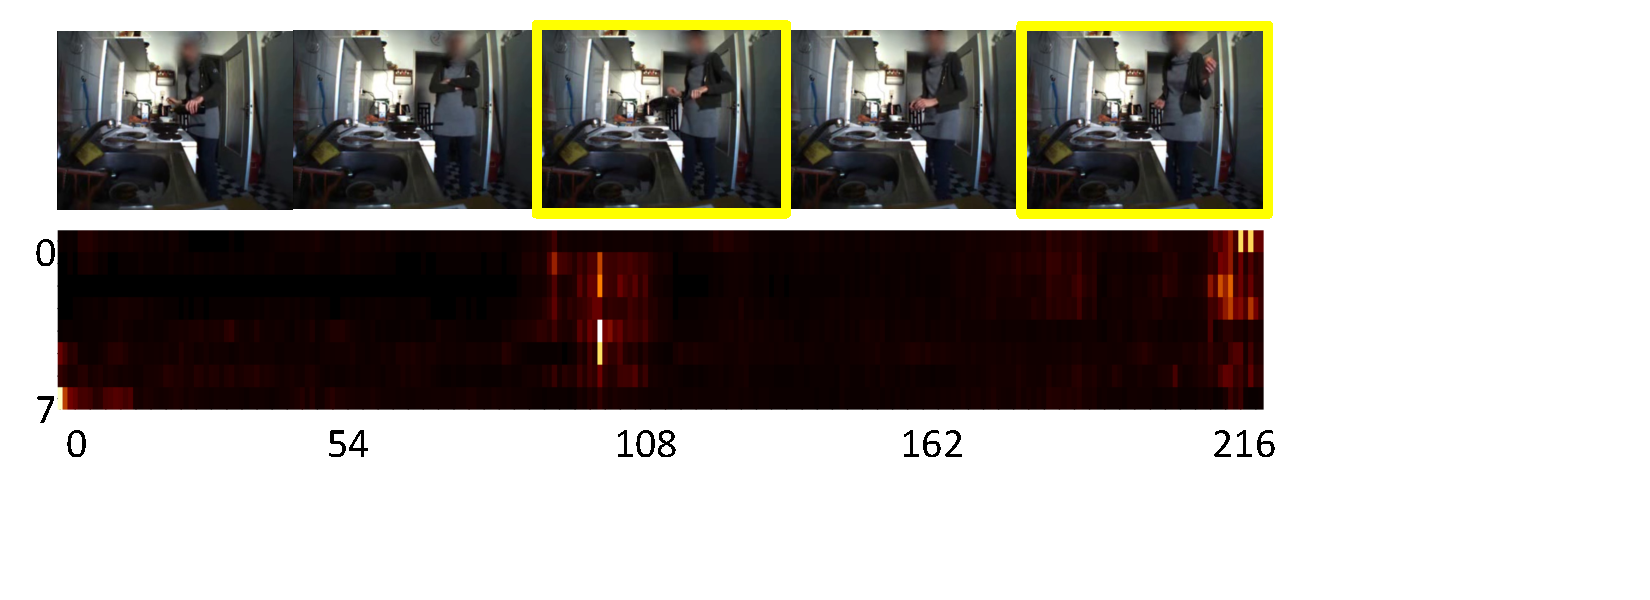
\includegraphics[width=\columnwidth]{Figures/pdf/attn_vis_fe2.pdf}
    \caption{Activity: Fried egg}
    \label{fig:4a}
    \end{subfigure}
    \begin{subfigure}[t]{\linewidth}
    % \vspace{1mm}
    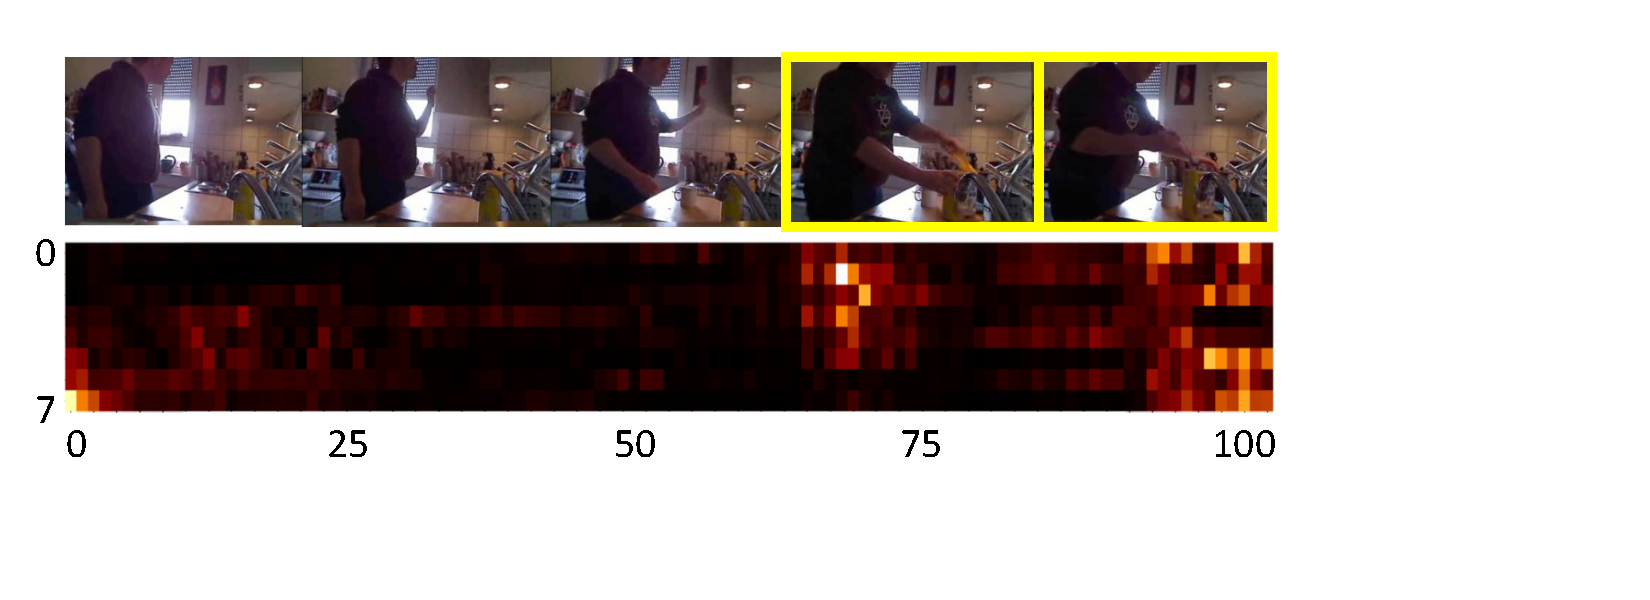
\includegraphics[width=\columnwidth]{Figures/pdf/attn_vis_milk2.pdf}
    \caption{Activity: Milk}
    \label{fig:4b}
    \end{subfigure}
\caption{\textbf{Cross-attention map visualization on Breakfast}. The horizontal and vertical axis indicates the index of the past frames and the action queries, respectively. The brighter color implies a higher attention score. We highlight a video frame with a yellow box where the attention score of the frame is highly activated. RGB frames are uniformly sampled from a video in this figure.}
 \label{fig:4}
\end{figure}
\begin{figure*}[t]
    \centering
    \begin{subfigure}[t]{\linewidth}
    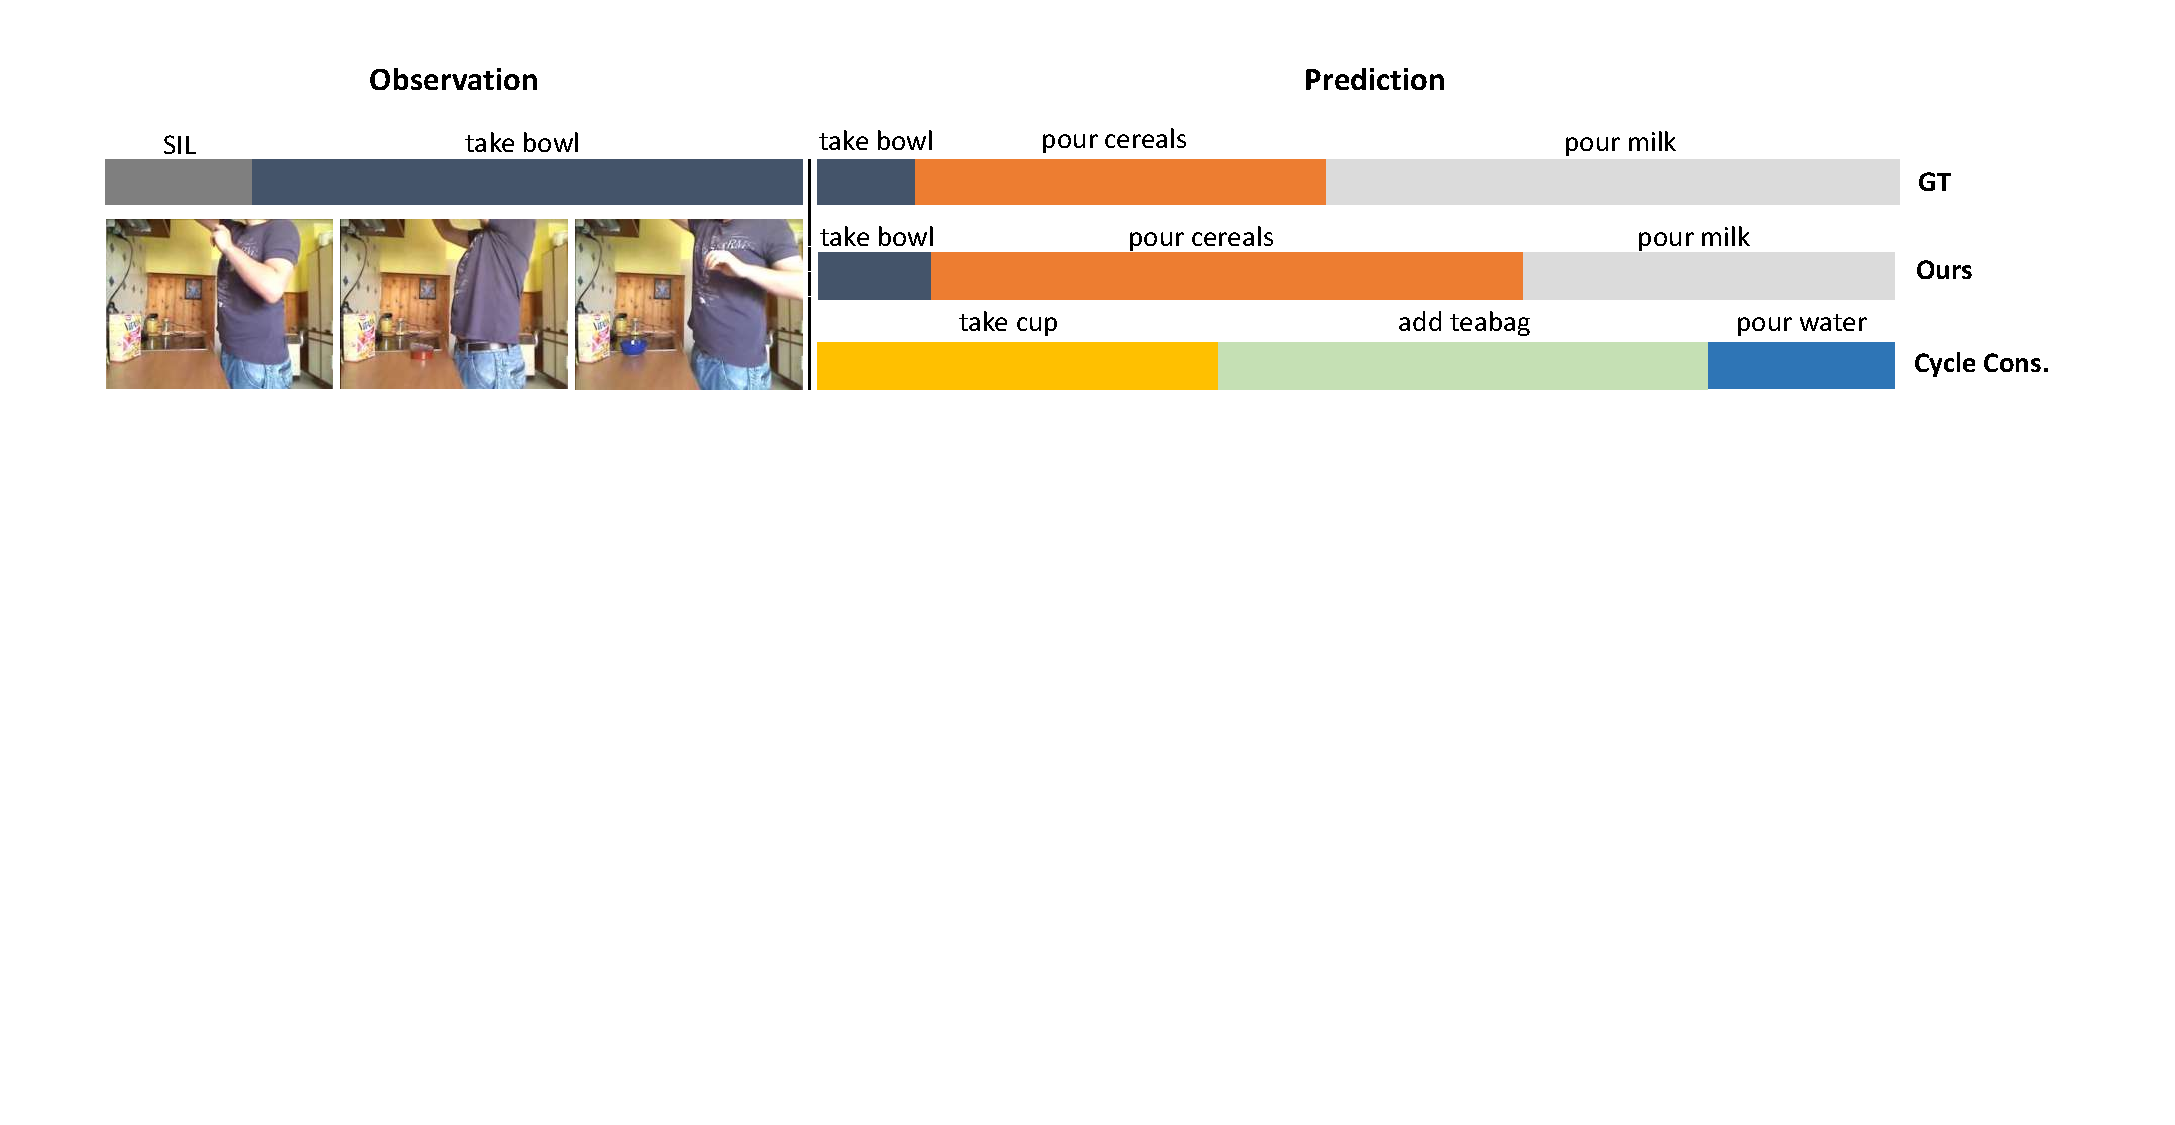
\includegraphics[width=\columnwidth]{Figures/pdf/qual_1_compressed.pdf}
    \caption{Activity: Cereal}
    \label{fig:5a}
    \end{subfigure}
    \vspace{-1mm}
    \begin{subfigure}[t]{\linewidth}
    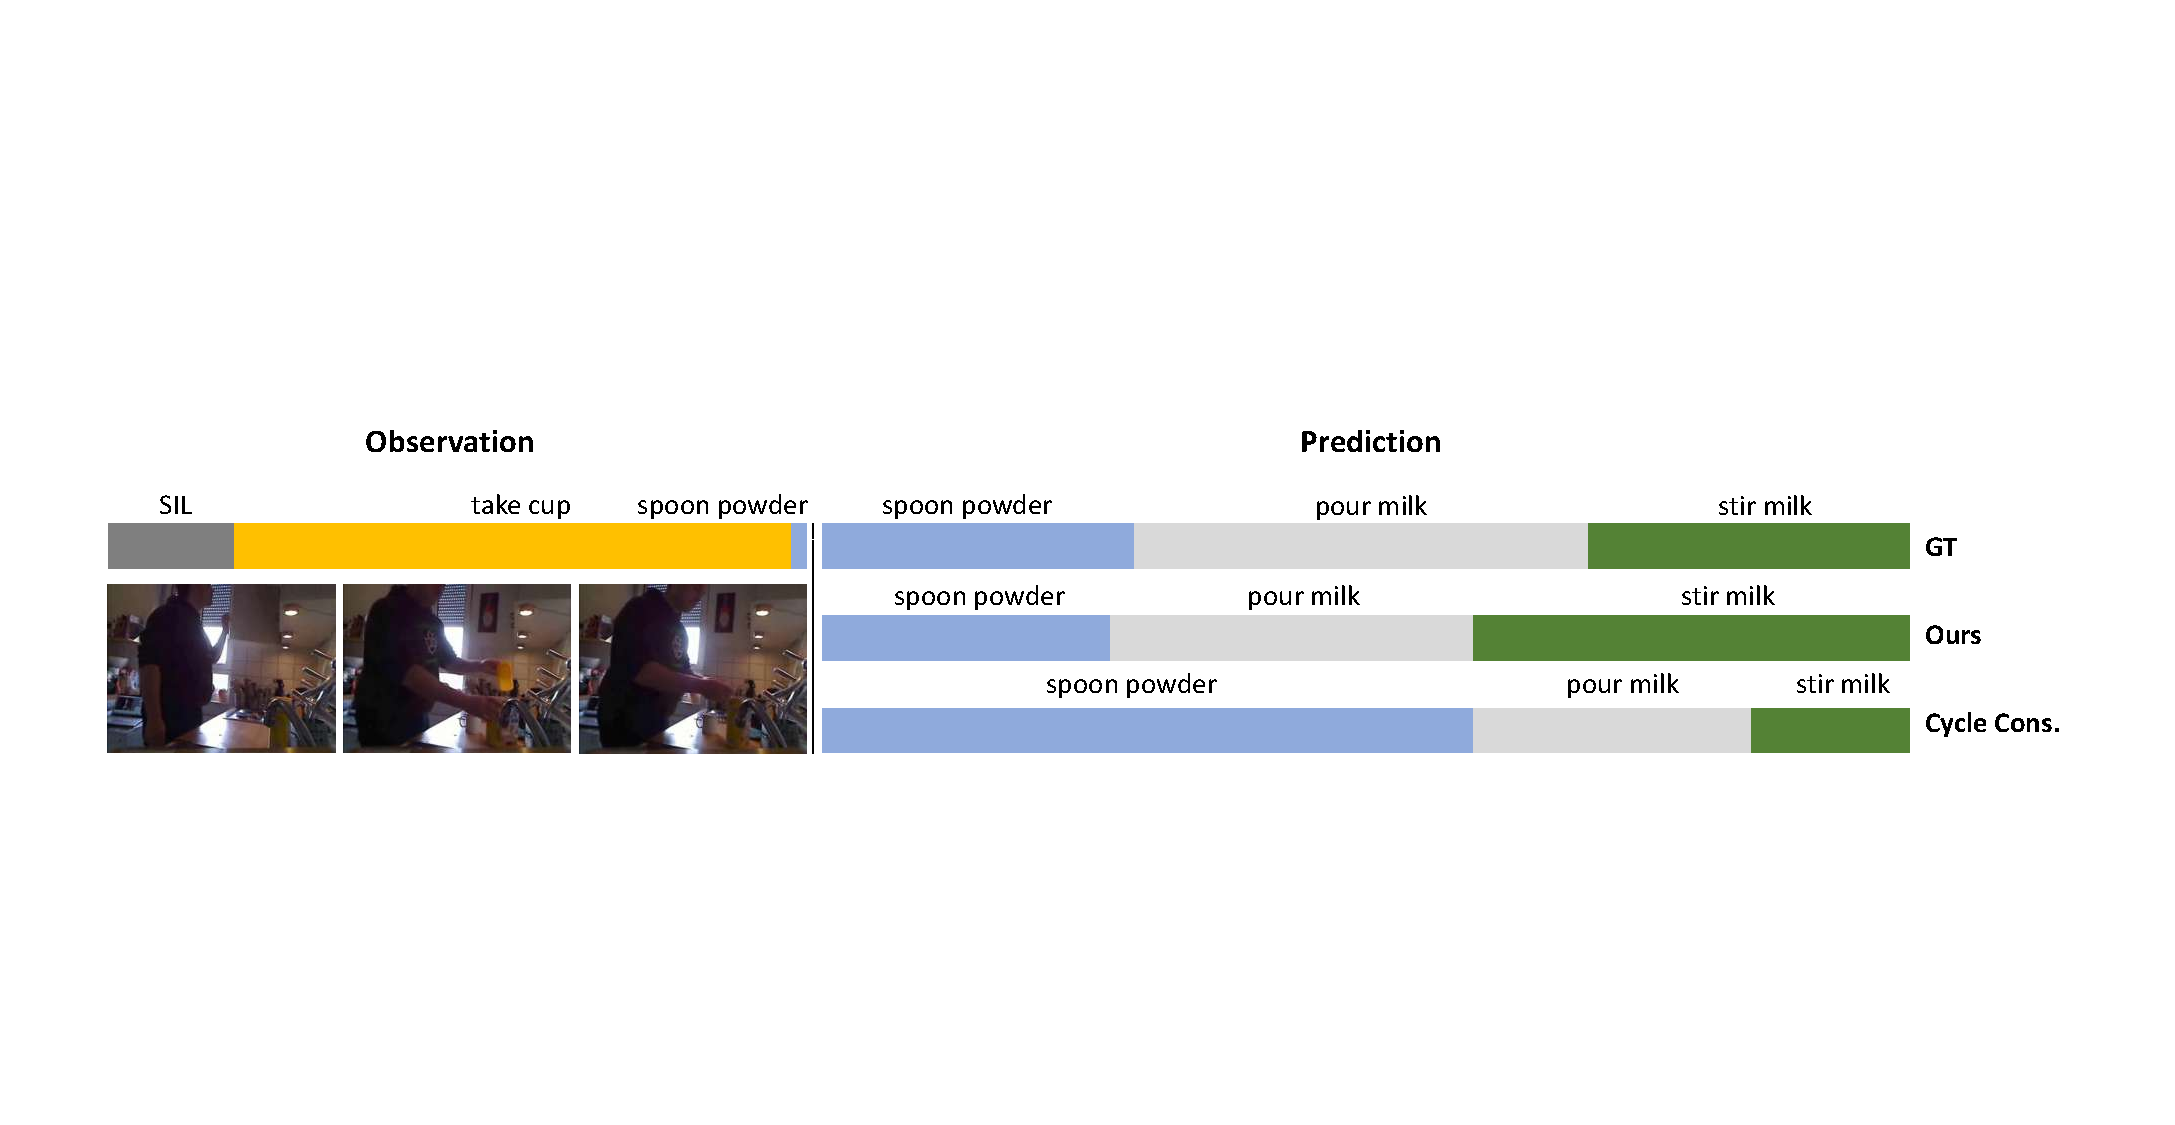
\includegraphics[width=\columnwidth]{Figures/pdf/qual_2_compressed.pdf}
    \caption{Activity: Milk}
    \label{fig:5b}
    \end{subfigure}
    \vspace{-1mm}
    \begin{subfigure}[t]{\linewidth}
    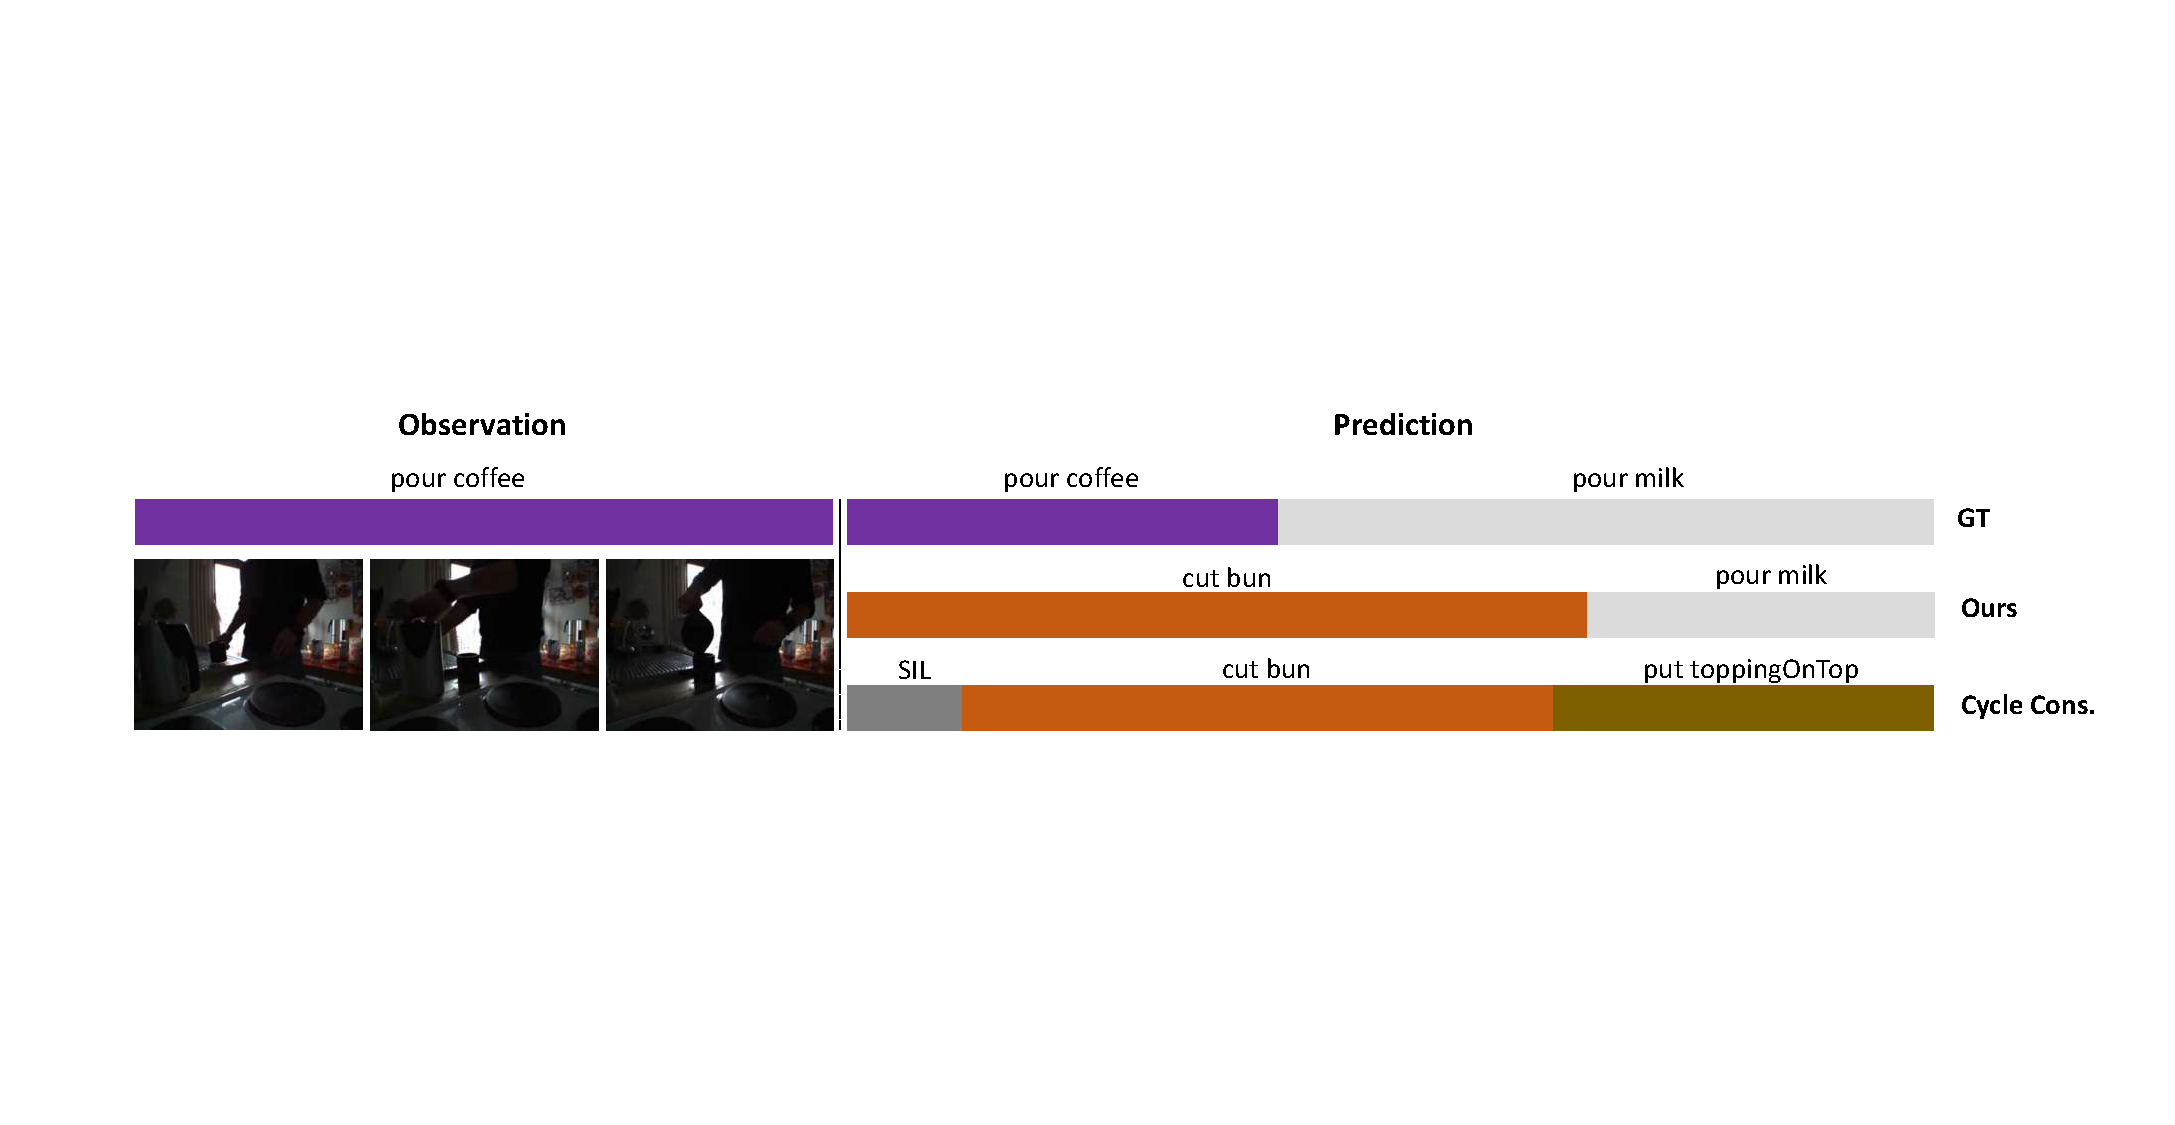
\includegraphics[width=\columnwidth]{Figures/pdf/qual_3_compressed.pdf}
    \caption{Activity: Coffee}
    \label{fig:5c}
    \end{subfigure}
\caption{\textbf{Qualitative results on Breakfast}. Each subfigure visualizes the ground-truth labels and predicted results of the \ours and the Cycle Cons.~\cite{farha2020long}. We set $ \alpha $ as 0.3 and $ \beta $ as 0.5 in this experiment. We decode action labels and durations as frame-wise action classes. Each color in the color bar indicates an action label written above.}
\vspace{-4mm}
 \label{fig:5}
\end{figure*}
\begin{table}[t!]
\begin{center}
\scalebox{0.9}{
\begin{tabular}{C{1.3cm}C{1.4cm}C{1.4cm}C{1.4cm}C{1.4cm}}
        \toprule
        \multirow{2}*[-0.5ex]{$M$}& \multicolumn{4}{c}{$\beta~(\alpha=0.3)$} \\ 
        \cmidrule( l){2-5}
        & 0.1 & 0.2 & 0.3 & 0.5 \\
        \cmidrule{1-5}
        6 & 29.95 & 26.47 & 25.46 & 23.27 \\
        7 & 30.03 & 27.94& 27.00 & 24.23 \\
        \ccolg 8 & \ccolg \textbf{32.27} & \ccolg \textbf{29.88} &  \ccolg 27.49 & \ccolg \textbf{25.87}\\
        9 & 31.24 & 28.65& 26.87 & 24.95 \\
        10 & 31.32 & 28.86& \textbf{27.74} & 25.01 \\
        \bottomrule
        \end{tabular}}
\end{center}
\vspace{-2mm}
\caption{\textbf{Number of action queries.} We adjust the number of action queries $M$, showing that a sufficient number of action queries shows saturated performance. }
\vspace{-4mm}
\label{tab:query}
\end{table}

% C{1.3cm}C{1.4cm}C{1.4cm}C{1.4cm}C{1.4cm}
% C{1.2cm}C{1.2cm}C{1.2cm}C{1.2cm}C{1.2cm}

\vspace{2mm}

\noindent
\textbf{Number of action queries.}
To analyze the impact of the number of action queries $M$ in \ours, we adjust the value of $M$ from 6 to 10. In Table~\ref{tab:query}, the performance becomes saturated as we gradually increase the number of action queries. By this experiment, we set $M$ to 8 for Breakfast.

See Supp.~C and D for additional analysis and results.

\subsection{Attention map visualization}
We visualize the cross-attention layers in the decoder in Fig.~\ref{fig:4}. The vertical and horizontal axis indicates the index of the action queries and input past frames, respectively. 
We find two interesting results from this experiment.
First, our model learns to attend to visual features in the recent past, showing that the nearest frames provide crucial keys for predicting future actions. 
It is in alignment with the previous work~\cite{ke2019time,sener2020temporal} that reflects the importance of the recent past in designing anticipation models.
\ours also attends to the recent past without any prior knowledge applied to the model.
Second, we find that \ours is trained to attend to important actions not only from the recent past, but also from the entire past frames. In Fig.~\ref{fig:4a}, essential frames with yellow boxes are detected by the queries with the high attention scores, providing contextual clues of the activity,~\eg `holding a pan' and `taking an egg' actions in the `fried egg' activity. Furthermore, action queries anticipating \textit{NONE} class attend to the irrelevant features such as the beginning of the videos. The results show that \ours effectively leverages long-term dependencies using the entire past frames regardless of the position, and also detects key frames of the given activity.
More visualization results are shown in Supp.~E.

\subsection{Qualitative results}
Figure~\ref{fig:5} shows the qualitative results of \ours and Cycle Cons.~\cite{farha2020long}, evaluating on long-term action anticipation. In this experiment, we plot the prediction results based on the a sequence of predicted action label and corresponding duration. Each subfigure consists of observed frames, the ground-truth~(GT) labels, and prediction results from the two models. Observed frames are uniformly sampled from videos.
Figure~\ref{fig:5a} shows the importance of utilizing fine-grained features for action anticipation. 
\ours anticipates `take bowl' action from the observed frames, while Cycle Cons. model anticipates `take cup' action missing fine-grained features, which leads to the error accumulation of the rest of the predictions.
Figure~\ref{fig:5c} validates the robustness of parallel decoding on error accumulations from the previous predictions. Although the two models were wrong in the first anticipation, our model correctly predicts the following action label while Cycle Cons. generates false results during iterative predictions.
The results also validates effectiveness of the proposed methods on various activities.
See Supp.~E for more qualitative results.